\subsection{Thực hành}
\subsubsection{HOG+SVM}
Bài toán áp dụng phương pháp HOG+SVM được thực hiện thông qua ba giai đoạn: tiền xử lý dữ liệu, training và detecting.

Với giai đoạn traning, mô hình sẽ được huấn luyện qua các bước:
\begin{itemize}[noitemsep, topsep=0pt, leftmargin=1.25em, label={$-$}]
    \item Bước 1: Chuẩn bị dữ liệu đào tạo.
    \item Bước 2: Trích xuất đặc trưng HOG.
    \item Bước 3: Huấn luyện SVM phân loại hình ảnh trong bộ dữ liệu đào tạo.
\end{itemize}

Đối với giai đoạn detecting:
\begin{itemize}[noitemsep, topsep=0pt, leftmargin=1.25em, label={$-$}]
    \item Bước 1: Chuẩn bị dữ liệu test khác với dữ liệu đào tạo.
    \item Bước 2: Sử dụng sliding windows trượt qua từng vùng ảnh.
    \item Bước 3: Trích xuất đặc trưng HOG trong từng vùng ảnh.
    \item Bước 4: Phân loại với mô hình SVM đã được đào tạo trong phần training.
\end{itemize}

Có thể hình dung 2 giai đoạn trên qua hình ảnh dưới đây \cite{HOG&SVMped}:   
\graphicspath{{figures/}}
\begin{figure}[h!]
  \centering
  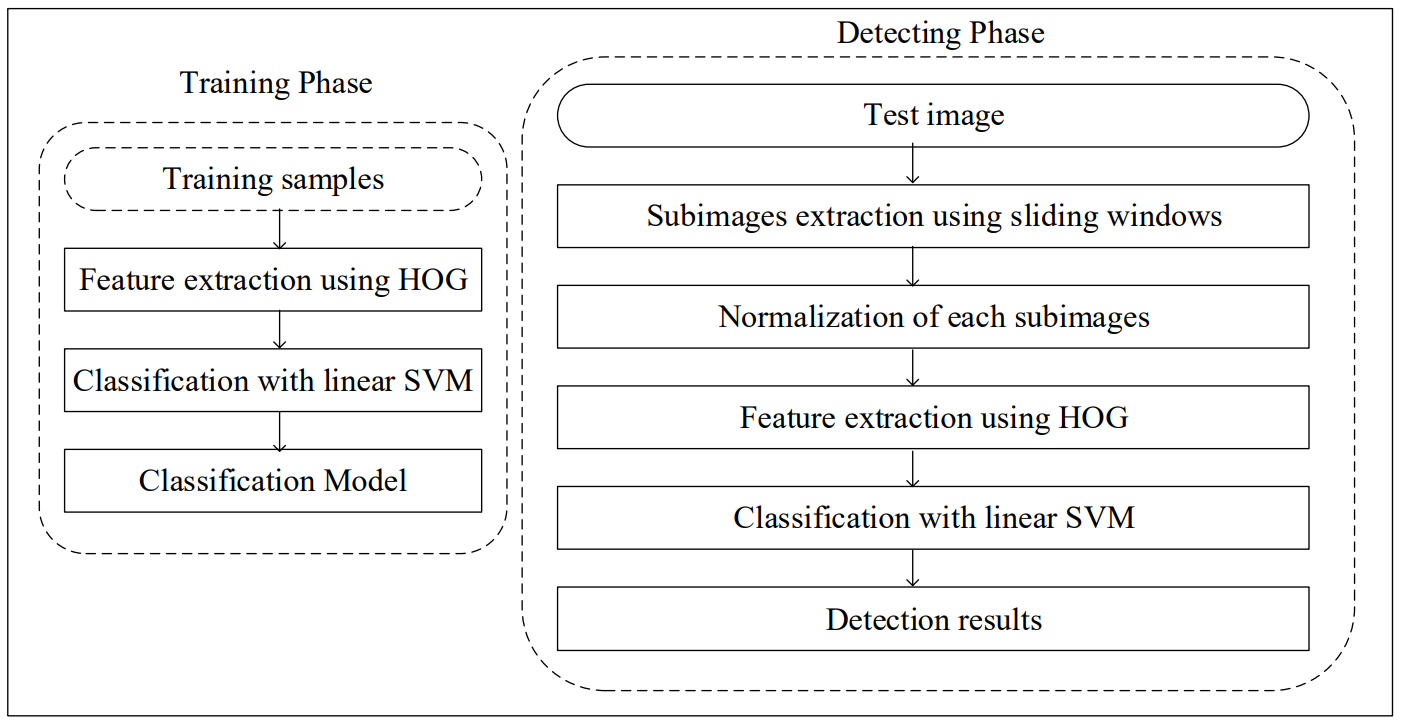
\includegraphics[scale=0.4]{graphics/detectingphaseofHOGSVM.png}
  \caption{Tóm tắt hai giai đoạn traning và detecting của model HOG+SVM.}
\end{figure}

Để hiểu rõ hơn về các bước ở mỗi giai đoạn, chúng ta sẽ đi vào chi tiết qua từng mục dưới đây.
\paragraph{Giai đoạn tiền xử lý dữ liệu\\}
Dataset sử dụng chứa các bức ảnh chứa ít nhất một người đi bộ. Tuy nhiên, vì HOG+SVM là một phương pháp sử dụng mô hình phân loại, chúng ta cần tạo ra tập positive và negative sample set từ dữ liệu huấn luyện. Trong trường hợp này, ta sử dụng 170 bức ảnh trong dataset và có 345 người đi bộ đã được dán nhãn từ dataset.

\textbf{Tạo positive samples} - Đầu tiên, ta đọc các ảnh từ dataset và bounding box (hộp giới hạn) đã được cung cấp. Bước tiếp theo là sử dụng bounding box như ranh giới để lấy các vùng có diện tích bên trong bounding box làm positive sample. Các positive sample này được lưu vào thư mục positive samples. Positive samples là các vùng trong ảnh được xác định là chứa người đi bộ.

\textbf{Tạo negative samples} - Tương tự như bước trước, ta đọc các ảnh từ dataset. Sử dụng hàm detectMultiScale của HOG để xác định các vùng chứa người đi bộ. Với mỗi vùng đã xác định, ta sử dụng sliding window để duyệt qua từng vùng trên từng ảnh đầu vào. Nếu vùng đó trùng với bounding box của detectMultiScale, ta bỏ qua vùng đó và tiếp tục với vùng khác. Ngược lại, nếu vùng không trùng với bounding box, ta lấy vùng đó làm ảnh nền/negative sample. Các negative sample này sau đó được lưu vào thư mục negative samples. Negative samples là các vùng trong ảnh không chứa người đi bộ. Do số lượng negative samples rất lớn so với positive samples, nhóm đã giới hạn lại số lượng negative samples là 800.

\graphicspath{{figures/}}
\begin{figure}[h!]
  \centering
  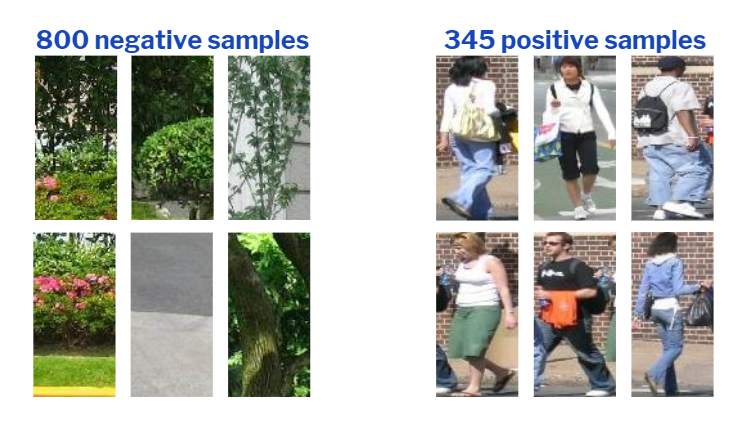
\includegraphics[scale=0.5]{graphics/data-prep.png}
  \caption{Kết quả của giai đoạn tiền xử lí dữ liệu}
\end{figure}

Qua giai đoạn tiền xử lí dữ liệu này, nhóm đã tạo thành hai tập dữ liệu con: positive samples và negative samples. Tỉ lệ của positive và negative samples lần lượt là 345 và 800, tạo ra tập dữ liệu mất cân bằng (imbalanced dataset). Tuy vậy tỉ lệ này lại sát với thực tế, khi mà số lượng người đi bộ trong các bức ảnh là không nhiều và phần lớn vùng diện tích của bức ảnh là nền. Các tập dữ liệu này sẽ được sử dụng trong giai đoạn huấn luyện mô hình SVM để phân loại và nhận dạng người đi bộ trong ảnh.
\paragraph{Giai đoạn training\\}
Trong phần này, model SVM sẽ được training qua chi tiết các bước:
\begin{itemize}[noitemsep, topsep=0pt, leftmargin=1.25em ]
    \item Bước 1: Chuẩn bị dữ liệu:
    \begin{itemize}[noitemsep, topsep=0pt, leftmargin=1.5em, label={$-$}]
        \item Thu thập tập dữ liệu chứa các ảnh với người đi bộ và các ảnh không chứa người đi bộ với kích thước 64x128 như phần tiền xử lý dữ liệu đã nói phía trên.
        \item Gán nhãn dữ liệu: 800 tấm ảnh negative sẽ được gán nhãn là 0, 345 tấm ảnh người positive được gán nhãn là 1.
    \end{itemize}
    \item Bước 2: Trích xuất đặc trưng HOG:
    \begin{itemize}[noitemsep, topsep=0pt, leftmargin=1.5em, label={$-$}]
        \item Sử dụng phương pháp HOG (Histogram of Oriented Gradients) để trích xuất đặc trưng từ các hình ảnh trong bộ dữ liệu đào tạo.
    \end{itemize}
    \item Bước 3: Huấn luyện SVM phân loại hình ảnh trong bộ dữ liệu đào tạo:
    \begin{itemize}[noitemsep, topsep=0pt, leftmargin=1.5em, label={$-$}]
        \item Kết hợp hai bộ ảnh đã được tính đặc trưng HOG là positive và negative lại với nhau để chia tập dữ liệu thành train và test. Với tỉ lệ 8:2 ta có được tập train là 915 hình ảnh và tập test là 230 hình ảnh.
        \item Sử dụng các đặc trưng HOG đã được trích xuất từ bước trước đó và nhãn tương ứng để huấn luyện một mô hình SVM với hai tập dữ liệu train và test.
    \end{itemize}
\end{itemize}

Sau giai đoạn traning, chúng ta sẽ có được model SVM đã train sử dụng nó để detect người đi bộ trong giai đoạn tiếp theo.
\paragraph{Giai đoạn deteting\\}
Với giai đoạn detecting, ta sẽ có thêm một số khái niệm cần chú ý, trước tiên ta sẽ đi qua chi tiết các bước:
\begin{itemize}[noitemsep, topsep=0pt, leftmargin=1.25em ]
    \item Bước 1: Chuẩn bị dữ liệu test khác với dữ liệu đào tạo:
    \begin{itemize}[noitemsep, topsep=0pt, leftmargin=1.5em, label={$-$}]
        \item Dữ liệu test cho phần phát hiện đối tượng này là các hình ảnh chứa 1 hoặc nhiều người đi bộ để kiểm tra model phát hiện người đi bộ trong hình ảnh.
    \end{itemize}
    \item Bước 2: Sử dụng \textbf{sliding windows} trượt qua từng vùng ảnh:
        \begin{itemize}[noitemsep, topsep=0pt, leftmargin=1.5em, label={$-$}]
            \item Áp dụng kỹ thuật \textbf{sliding windows} để chia nhỏ các hình ảnh trong bộ dữ liệu test thành các vùng nhỏ có kích thước 64x128.
            \item \textbf{Sliding windows} - là kĩ thuật sử dụng để quét qua toàn bộ hình ảnh bằng cách di chuyển một cửa sổ trượt có kích thước cố định qua từng vị trí trên ảnh, sau đó tăng kích thước cửa sổ với tỷ lệ được định nghĩa rồi tiếp tục quét cho đến khi kích thước cửa sổ được tăng bằng với kích thước ảnh. Bắt đầu từ góc trên bên trái của ảnh, cửa sổ trượt được di chuyển qua từng vị trí trên ảnh một cách tuần tự. Cửa sổ có thể được di chuyển theo bước nhảy (stride) cố định hoặc bước nhảy có thể được điều chỉnh tùy thuộc vào yêu cầu của bài toán.
            \graphicspath{{figures/}}
                \begin{figure}[h!]
                  \centering
                  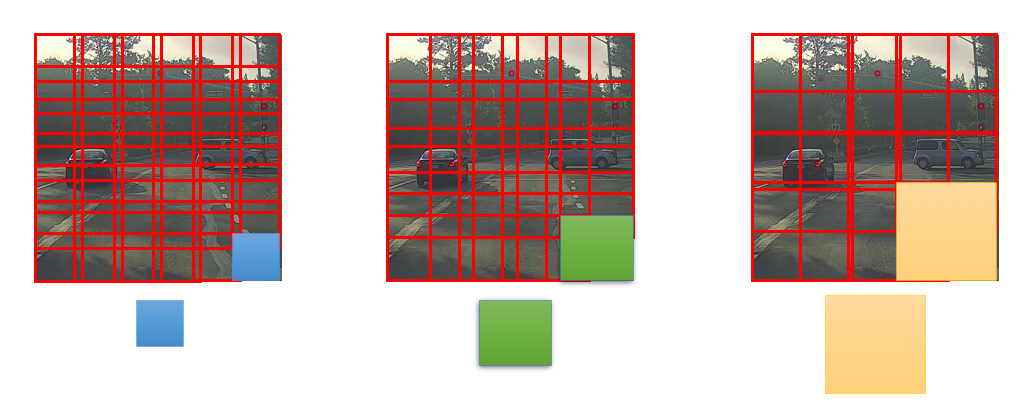
\includegraphics[scale=0.35]{graphics/slidingw.png}
                  \caption{Cách sliding window hoạt động trên một hình ảnh.}
                \end{figure}
            \item Việc chia nhỏ ảnh thành các vùng nhỏ này giúp xác định vị trí có thể xuất hiện người đi bộ trong ảnh.
        \end{itemize}
    \item Bước 3: Trích xuất đặc trưng HOG trong từng vùng ảnh:
    \begin{itemize}[noitemsep, topsep=0pt, leftmargin=1.5em, label={$-$}]
        \item Áp dụng phương pháp HOG để trích xuất đặc trưng từ từng vùng ảnh nhỏ thu được từ bước trước.
        \item Việc trích xuất đặc trưng HOG giúp tạo ra một biểu diễn số học của mỗi vùng ảnh, giúp phân loại xem có người đi bộ trong vùng đó hay không.
    \end{itemize}
    \item Bước 4: Phân loại với mô hình SVM đã được đào tạo trong phần training:
    \begin{itemize}[noitemsep, topsep=0pt, leftmargin=1.5em, label={$-$}]
        \item Sử dụng mô hình SVM đã được huấn luyện trong phần training để phân loại các vùng ảnh thu được từ bước trước. 
        \item Mô hình sẽ phân loại các ảnh con được quét qua bởi sliding window là ảnh nền hay ảnh con người theo những gì được học ở giai đoạn training.
    \end{itemize}
\end{itemize}
Quá trình trượt qua toàn bộ hình ảnh và áp dụng phân loại trên từng cửa sổ được lặp lại cho đến khi đã duyệt qua tất cả các vị trí trên ảnh. Cuối cùng, sử dụng kỹ thuật \textbf{non\_max\_suppression} để loại bỏ các khu vực overlap và chỉ giữ lại kết quả phân loại cuối cùng.
    \begin{itemize}[noitemsep, topsep=0pt, leftmargin=1.5em, label={$-$}]
        \item Một khái niệm nữa được dùng trong giai đoạn này đó là \textbf{non\_max\_suppression}. 
        \item \textbf{Non-maximum suppression (NMS)} - một kỹ thuật được sử dụng trong xử lý ảnh để loại bỏ trùng lặp và chọn lọc các đối tượng có độ tin cậy cao. Khi sử dụng kỹ thuật sliding window để phát hiện đối tượng trong ảnh, có thể xảy ra tình huống nhiều cửa sổ trượt chồng lấp lên nhau và phát hiện cùng một đối tượng. Điều này dẫn đến việc nhận dạng trùng lặp và tạo ra nhiều kết quả phát hiện không cần thiết. Để giảm hiện tượng này, ta sử dụng kỹ thuật non-maximum suppression.
        \graphicspath{{figures/}}
            \begin{figure}[h!]
            \centering
            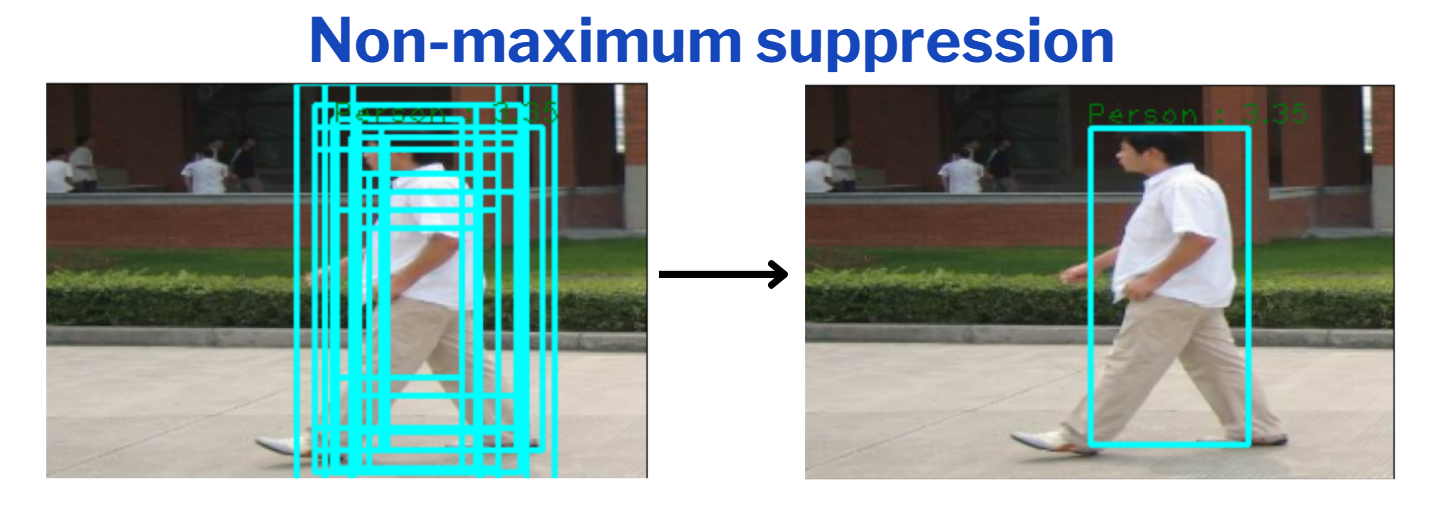
\includegraphics[scale=0.35]{graphics/NMS.png}
            \caption{NMS loại bỏ phát hiện dư trùng lặp, giữ lại phát hiện đáng tin cậy.}
        \end{figure}
    \end{itemize}
Cuối cùng, vẽ các hộp giới hạn xung quanh các khu vực dành cho người đi bộ được phát hiện và được xóa trùng lặp bởi NMS. Hình ảnh output nhận được sẽ là hình ảnh phát hiện người đi bộ bằng các bounding box bao quanh vùng phát hiện đó.

\subsubsection{Faster R-CNN}
\paragraph{Chuẩn bị bộ dữ liệu Penn-FundanFundan\\}

Phương thức getitem sẽ trả về: image là một PIL Image có kích thước (H, W) và target là một từ điển chứa các trường sau đây:
\begin{itemize}[noitemsep, topsep=0pt, leftmargin=1.25em, label={$-$}]
    \item boxes (FloatTensor[N, 4]): tọa độ của N bounding boxes trong định dạng [x0, y0, x1, y1], có giá trị từ 0 đến W và 0 đến H.
    \item labels (Int64Tensor[N]): nhãn cho mỗi bounding box. Giá trị 0 luôn đại diện cho lớp nền (background).
    \item image\_id (Int64Tensor[1]): một định danh hình ảnh. Nó là duy nhất giữa tất cả các hình ảnh trong bộ dữ liệu và được sử dụng trong quá trình đánh giá.
    \item area (Tensor[N]): Diện tích của bounding box được sử dụng trong quá trình đánh giá với các tiêu chí COCO, để phân tách điểm số tiêu chí cho các bounding box nhỏ, vừa và lớn.
    \item iscrowd (UInt8Tensor[N]): Các instance với iscrowd=True sẽ được bỏ qua trong quá trình đánh giá.
\end{itemize}
\begin{figure}[h!]
  \centering
  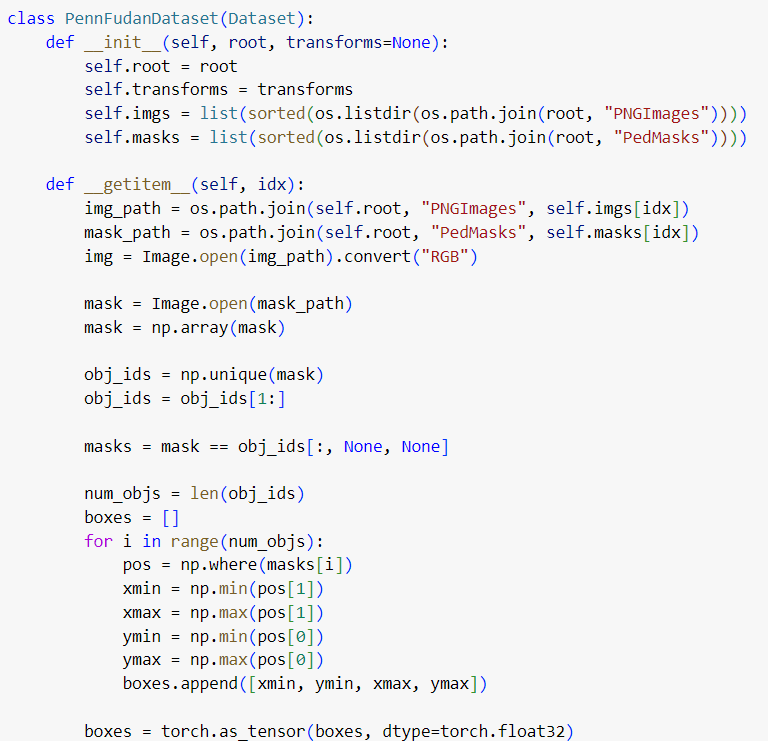
\includegraphics[scale=0.65]{graphics/loaddata.png}
  \caption{Hàm để load bộ dữ liệu Penn-Fundan}
\end{figure}
\pagebreak
\paragraph{Xây dựng mô hình\\}
Nhóm chúng em đã lựa chọn như sau:
\begin{itemize}[noitemsep, topsep=0pt, leftmargin=1.25em, label={$-$}]
    \item backbone: sử dụng mô hình mạng nơ-ron tiền huấn luyện MobileNetV2. Mô hình này sẽ được sử dụng để trích xuất đặc trưng từ ảnh đầu vào.
    \item AnchorGenerator được sử dụng để tạo ra các vùng đề xuất trên feature map để đề xuất các vùng có khả năng chứa đối tượng cao.
    \item MultiScaleRoIAlign được sử dụng để pooling features từ feature map theo vùng đề xuất (region of interest - ROI) để chuẩn bị đầu vào cho lớp classification và regression của mô hình.
    \item Faster R-CNN được cấu hình để nhận diện 2 lớp đối tượng: có người đi bộ và background (num\_classes=2)
\end{itemize}

\pagebreak

\begin{figure}[h!]
  \centering
  \subfloat{{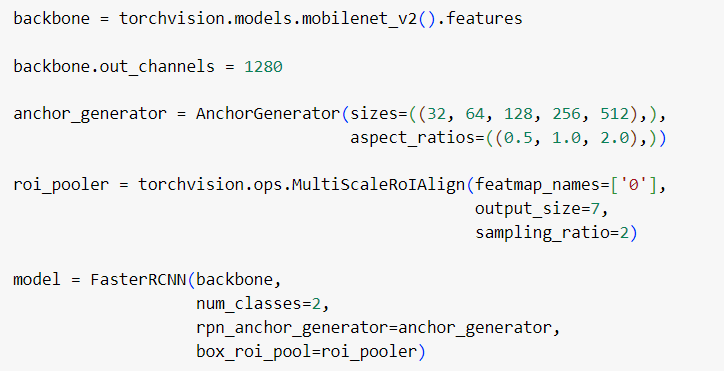
\includegraphics[scale=0.7]{graphics/backbone.png} }}
  \qquad
  \subfloat{{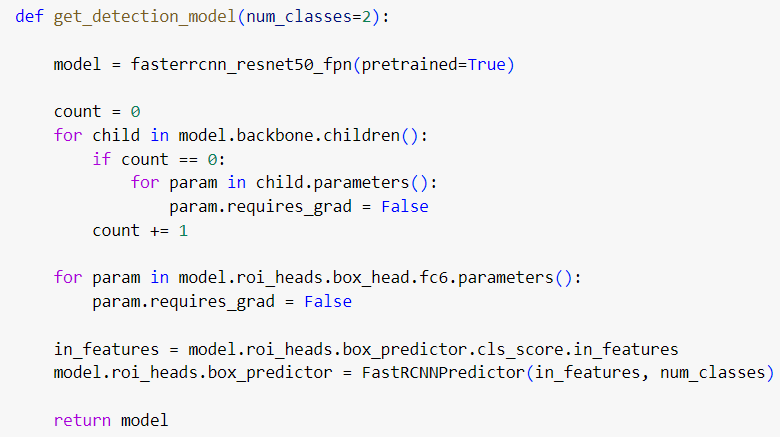
\includegraphics[scale=0.7]{graphics/model.png} }}
  \caption{Code xây dựng mô hình Faster R-CNN}
\end{figure}

Ta thực hiện hàm transform để biến đổi mỗi hình ảnh đầu vào sang định dạng phù hợp để mô hình các mạng nơ-ron của PyTorch có thể xử lý được. 
\begin{figure}[h!]
  \centering
  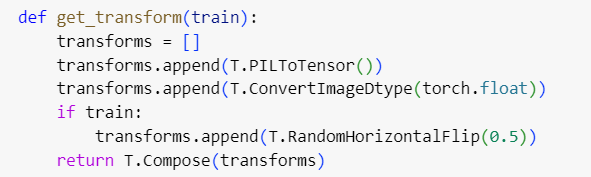
\includegraphics[scale=0.65]{graphics/transform.png}
  \caption{Hàm transform}
\end{figure}

\paragraph{Chia tập train và test\\}
Tiếp theo ta chia dataset thành hai tập train và test để sử dụng cho việc huấn luyện và đánh giá mô hình. Trong phần thực nghiệm này, nhóm chia với tỉ lệ 0.7 nghĩa là 70\% dữ liệu sử dụng cho tập huấn luyện.

\pagebreak

\begin{figure}[h!]
  \centering
  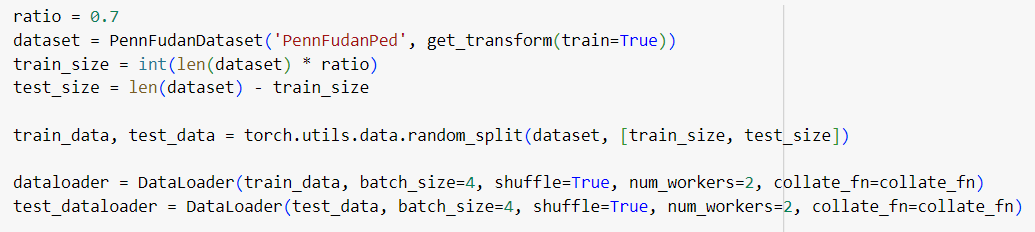
\includegraphics[scale=0.65]{graphics/split.png}
  \caption{Chia dataset bằng train\_test\_split}
\end{figure}

\paragraph{Lựa chọn các hyperparameters\\}
Ở phần này, nhóm chỉ sẽ thực nghiệm với các giá trị learning rate (lr) $\in \{0.004, 0.005, 0.006\}$ để đánh giá mô hình khi learning rate thay đổi trong các giá trị này. Các giá trị tham số khác được tham khảo từ thư viện PyTorch.
\begin{figure}[h!]
  \centering
  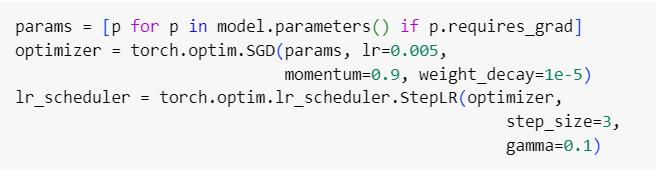
\includegraphics[scale=0.8]{graphics/params.png}
  \caption{Lựa chọn các hyperparameters}
\end{figure}

\paragraph{Huấn luyện mô hình\\}
Với mỗi epoch ta tính tổng giá trị loss và in ra để quan sát.
\begin{figure}[h!]
  \centering
  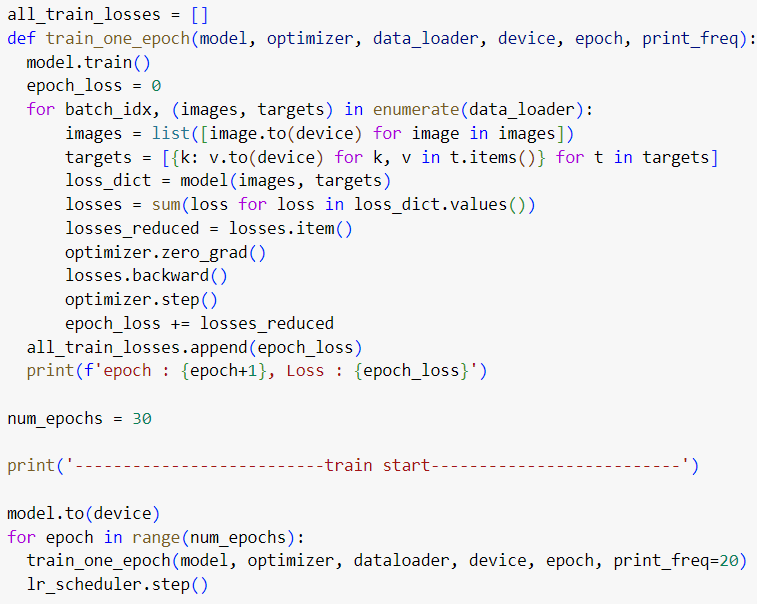
\includegraphics[scale=0.7]{graphics/train.png}
  \caption{Huấn luyện mô hình với 30 epochs}
\end{figure}